\section{Voltage Adaptor}
The purpose of this block is to convert 230 VAC from the electrical mains to a 12 VDC supply voltage. This voltage can then be used to power the various electrical components in the system. Some of the components can draw power directly from the 12 VDC line while other components requires even lower voltages.

\subsection{Analysis}
As the voltage Adaptor supplies every component in the system, it is important that it is rated to handle the amount of current which is drawn.
In order to calculate the minimum current rating:

\textbf{12 VDC components}\\
The only components which are directly supplied by the Voltage Adaptor are the Torque Sensor and the MOSFET-driver.

\begin{itemize}
	\item The Torque Sensors current consumption is rated to be $\leq  \SI{60}{\milli \ampere}$. For a worst-case analysis the maximum value is chosen:\\
	$I_{sensor} = \SI{60}{\milli \ampere}$
	\item Current drawn from the Torque Sensor by the PSoC:\\
	$I_{signal} = \SI{5}{\milli \ampere}$
	\item The current consumed by the MOSFET-driver's gate is calculated in section \vref{sec:LoadSystem} and will not be examined in this section. The amount of current consumed is calculated as:\\
	$I_{gate} = \SI{3.90}{\ampere}$
\end{itemize}

The total amount of current which is drawn at the 12 VDC line can be calculated as the sum of the component's current-consumptions:
\begin{equation}
	\begin{split}
		I_{12V} &= I_{sensor} + I_{signal} + I_{gate}\\
		I_{12V} &= \SI{60}{\milli \ampere} + \SI{5}{\milli \ampere} + \SI{3.90}{\ampere} = \SI{3.965}{\ampere}
	\end{split}
\end{equation}

\textbf{5 VDC components}\\
The amount of current consumed by the 5 VDC line is calculated in \vref{sec:LevelConverter} and will not be examined in this section. The amount of current consumed is calculated as:
\begin{equation}
	I_{5V} = \SI{613}{\milli \ampere}
\end{equation}

\textbf{Minimum rating}\\
The minimum amount of current which the adaptor must be able to deliver, can be found as the sum of currents drawn at the two voltage-levels:
\begin{align}
	\begin{split}
		I_{min} &= I_{5V} + I_{12V}\\
		I_{min} &= \SI{613}{\milli \ampere} + \SI{3.965}{\ampere} = \SI{4.578}{\ampere}
	\end{split}
\end{align}

This means that the system can be supplied by any 12 VDC voltage adaptor which is rated to deliver a minium of \SI{4.58}{\ampere}.

\subsection{Implementation}
The Voltage Adaptor is implemented using a GS60A12-P1J adaptor from Mean Well. This adaptor is rated to be able to deliver a current up to \SI{5.0}{\ampere} and gives a \SI{50}{\hertz} sinusoidal output. The adaptor connects the Control-box with the electrical mains with a \SI{2.1}{\milli \meter} coaxial plug. For safety reasons the Rolling Road circuit design also contains a \SI{5}{\ampere} fuse on the supply line. Furthermore, the voltage adaptor also supplies the Level Converter - this line is not protected with a fuse. The final design which is implemented on the print is seen on Figure \ref{fig:DesignVoltageAdaptor} below.

\begin{figure}[H]
	\centering
	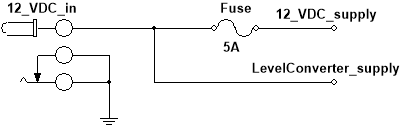
\includegraphics[width=0.5\linewidth]{Hardware/Pictures/DesignVoltageAdaptor}
	\caption{Implemented circuit design on Rolling Road}
	\label{fig:DesignVoltageAdaptor}
\end{figure}

\subsection{Unit test}
The Voltage Adaptor is tested using Analog Discovery's built-in oscilloscope. The average output-voltage is found to be \SI{11.998}{\volt}. The output is seen below.

\begin{figure}[H]
	\centering
	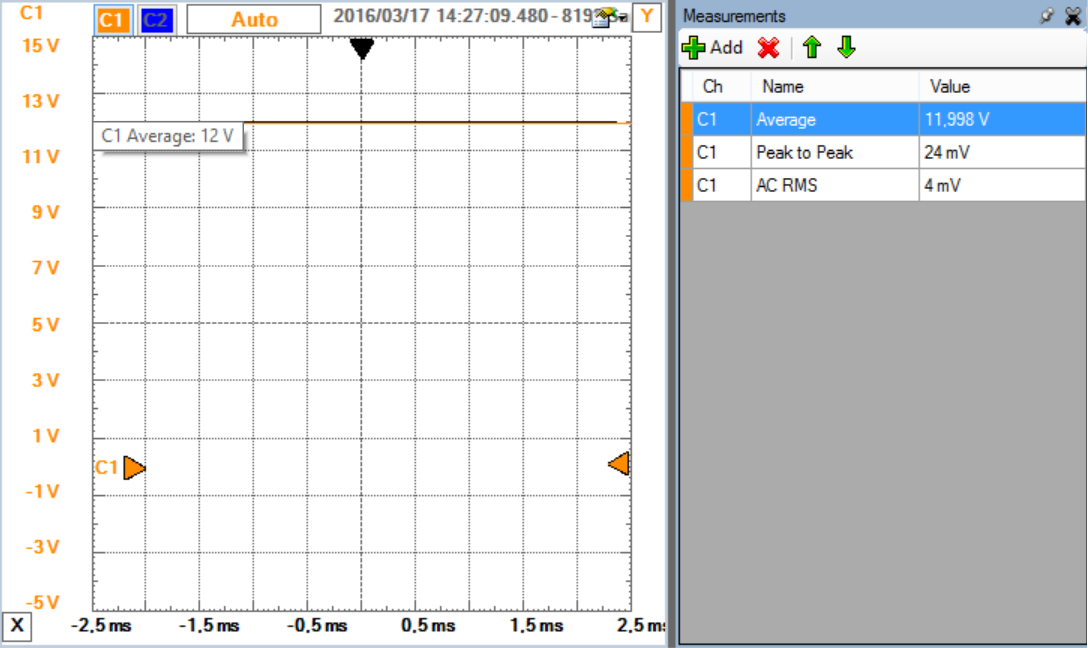
\includegraphics[width=0.9\linewidth]{Hardware/Pictures/VoltageAdaptor_test}
	\caption{Voltage Adaptor output over time}
	\label{fig:VoltageAdaptor_test}
\end{figure}